\begin{figure}
	{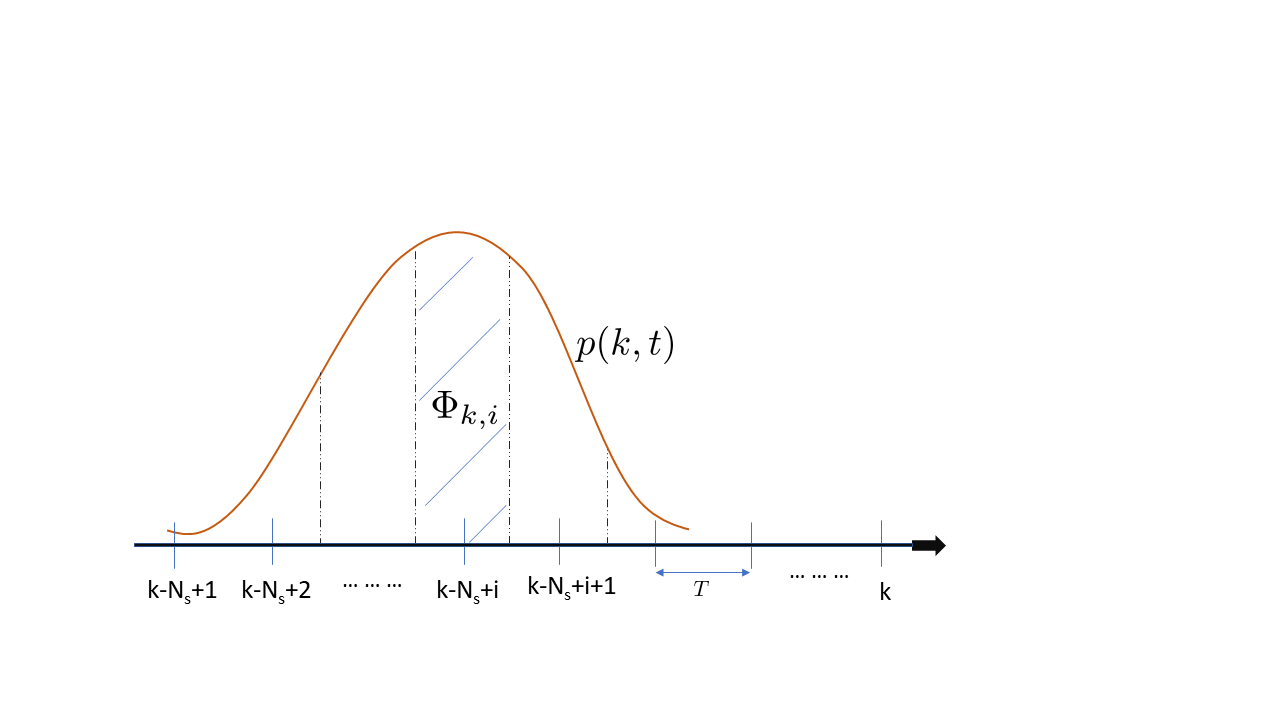
\includegraphics[width=1.0\columnwidth]{./img/delay_uncertainty.png}}
	\caption{Uncertianty of delay}
	\label{fig:delay_uncertainty}
\end{figure}

This section will describe the state estimation approach for the linear system in eqns. (\ref{eqn:LinearStateProp}) and (\ref{eqn:LinearUndelayedMeasurement}), along with time delayed measurements modelled in eqn. (\ref{eqn:LinearDelayedMeasurement}), which are corrupted by unknown bias $\Boldb_k$. 
For the derivation of the approach described in this section the reader is advised to refer to Section IV in \cite{choi2012state}.

It is essential to know the value of bias to migitate its effect on the posterior estimate of the state. Since it's not known prior to the estmiation, $\Boldb_k$ is simultaneously estimated along with the state. 
Assume that state vector at time $k$ is represented by $\Boldxi_k$.
The simultaneous estimation of the state \& the bias is achieved by performing estimation over an updated state vector defined as 
$
	\Boldx_k =
	\begin{bmatrix}
		\Boldxi_k^\top & \Boldb_k^\top
	\end{bmatrix}^\top. 
$

For the updated state vector, the linear time propagation model of eqn. (\ref{eqn:LinearStateProp}) can be rewritten as
\begin{align}
	\label{eqn:LinearStateProp4UpdatedState}
	\Boldx_{k+1} &\doteq \BoldF \Boldx_k + \BoldGamma \Boldw_k,
\end{align}

the linear measurement models in eqns. (\ref{eqn:LinearDelayedMeasurement}) and (\ref{eqn:LinearUndelayedMeasurement}) can be rewritten as
\begin{align}
	\label{eqn:LinearDelayedMeasurement4UpdatedState}
	\Boldz_k &\doteq \Big[ \BoldH_{k-N} \ \ \BoldI_{m_d} \Big] \Boldx_{k-N} +\Boldzeta_k \\
	\label{eqn:LinearUndelayedMeasurement4UpdatedState}
	\Boldy_k &\doteq \Big[ \BoldC_k \ \ \0_{m_u \times m_d} \Big] \Boldx_k + \Boldeta_k
\end{align}


The probability density function (PDF) $p(t)$ of the delay is assumed to be a known. As shown in figure (\ref{fig:delay_uncertainty}) the pdf is assumed to span over $\check{N}$ time steps. This assumption assigns a probability for correspondence of the delayed measurement $\Boldz_k$ with each of the time steps within time step $k$ and $k- \check{N}$.
Correspondence $r(k,i)$, $\forall i \in \{0, \dots, \check{N}\}$, signifies that measurement $\Boldz_k$ was induced by the state $\Boldx_{k-\check{N}+i}$.
The probability of correpondence $r_i$ is computed as
\begin{align}
	\Phi_{k,i} &= P(r(k,i)) \\
	&= P(t_l \le t \le t_u) \\
	&= \int_{t_l}^{ t_u} p(t) dt,
\end{align}
where $t_l = {j\tau - \frac{\tau}{2}}$, $t_u = {j \tau + \frac{\tau}{2}}$, $j = k - \check{N} + i $, $P(\cdot)$ denotes probability and $p(\cdot)$ denotes pdf of the time delay. When the PDF of the delay is specified, the maximum delay $\check{N}$ can be calculated using the cmulative distribution function (CDF) of the PDF. 
A value of $\check{N}$ should be chosen such that CDF of the time delay exceeds a given threshold. 
%A higher threshold value 99.6\% will ensure that the state $\Boldx_s$, where $k-\check{N} \le s \le k$, which induced the delayed measurement $\Boldz_k$ .
Choi et. al. have shown that probability of the correspondence $r_i$ for the given measurment $\Boldz_k$ is \cite{choi2012state}
\begin{align}
	P(r(k,i) | \Boldz_k ) = P(r(k,i)) = \Phi_{k,i}
\end{align}

Then, the optimal state estimator is
\begin{align}
	\hat{\Boldx}_k = \sum_{i=0}^{\check{N}} \Phi_{k,i} \hat{\Boldx}_{k,i},
\end{align}
where $\hat{\Boldx}_{k,i}$ is the estimation posterior computed the state estimate $\hat{\Boldx}_j^+$ computed in eqn. (\ref{eqn:posterior_state_estimate}), where $j = k - \check{N} + i$.

The optimal covariance matrix of the estimate is
\begin{align}
	\BoldP_k = \sum_{i = 0}^{\check{N}} \Phi_{k,i} [\BoldP_{k,i} + \hat{\Boldx}_k \hat{\Boldx}_k^\top] - \hat{\Boldx}_k \hat{\Boldx}_k^\top	
\end{align}
where $\BoldP_{k,i}$ is $a~posteriori$ state covariance matrix $P_j^+$ computed in eqn. (\ref{eqn:posterior_state_covar}),  where $j = k - \check{N} + i$. $\check{N}$



